\documentclass[11pt]{homework}

% TODO: replace these with your information
\newcommand{\hwname}{ZHOU Yuming}
\newcommand{\hwemail}{\href{mailto://121050081@link.cuhk.edu.cn}{121050081@link.cuhk.edu.cn}}
\newcommand{\hwtype}{Homework}
\newcommand{\hwnum}{1}
\newcommand{\hwclass}{MAT2040-T13}
\newcommand{\hwlecture}{0}
\newcommand{\hwsection}{Z}

% DEFINE ADDITIONAL MACROS
\newcommand\note{\textit{Note:\hspace{0.75cm}}}
\newcommand{\TODO}{\colorbox{red}{NOT DOING YET!}}
\newcommand{\claim}{\textit{\frame{Claim:}\hspace{0.75cm}}}
\newcommand{\recall}{\textit{\frame{Recall:}\hspace{0.75cm}}}

\usepackage{fontspec}
\defaultfontfeatures{Mapping=tex-text,Scale=MatchLowercase}
%\setmainfont{OpenDyslexic3}
\setmainfont{Atkinson Hyperlegible}
\setmonofont{Meslo LG L for Powerline}
% \crefname{questionCounter}{Good}{Note}

% Used for automatic embracing the text with brackets
\usepackage{xstring}

% DEFINE MATH MACROS
% \newcommand{\qed}{\hfill\rule{2mm}{2mm}}
\DeclareMathOperator*{\argmax}{arg\,max}
\DeclareMathOperator*{\argmin}{arg\,min}
\DeclareMathOperator*{\LHS}{LHS}
\DeclareMathOperator*{\RHS}{RHS}
\newcommand{\floor}[1]{\lfloor #1 \rfloor}
\newcommand{\ceil}[1]{\lceil #1 \rceil}
\newcommand{\myrightarrow}[1]{\mathrel{\raisebox{-2pt}{$\xrightarrow{#1}$}}}


% Other commands
\newcommand\st{\quad\text{s.t.}\quad}
\newcommand\E{\mathbb{E}} % expectation
\newcommand\F{\mathbb{F}} % fields
\newcommand\R{\mathbb{R}} % real
\newcommand\Q{\mathbb{Q}} % quadratic
\newcommand\Z{\mathbb{Z}} % integer
\newcommand\N{\mathbb{N}} % natural
\newcommand\bbC{\mathbb{C}} % complex
\newcommand\bbI{\mathbb{I}} % index function
\newcommand\bbS{\mathbb{S}}
\newcommand\calR{\mathcal{R}} % integrability
\newcommand\calF{\mathcal{F}} % family
\newcommand\calA{\mathcal{A}} % algebra
\newcommand\calB{\mathcal{B}} % Borel algebra
\newcommand\calM{\mathcal{M}}
\newcommand\bfi{\mathbf{i}}
\newcommand\bfj{\mathbf{j}}
\newcommand\bfk{\mathbf{k}}
\newcommand{\diam}{\operatorname{diam}}
\newcommand{\sumin}{\sum_{i=1}^n}
\newcommand{\sumiN}{\sum_{i=1}^N}
\newcommand{\sumiM}{\sum_{i=1}^M}
\newcommand{\sumjn}{\sum_{j=1}^n}
\newcommand{\sumjm}{\sum_{j=1}^m}
\newcommand{\sumil}{\sum_{i=1}^\ell}
\newcommand{\intab}{\int_{a}^{b}}

% Algebra
\newcommand{\GL}{\operatorname{GL}}
\newcommand{\SL}{\operatorname{SL}}
\newcommand{\Sym}{\operatorname{Sym}}
\newcommand{\lcm}{\operatorname{lcm}}
\newcommand{\sgn}{\operatorname{sgn}}
\newcommand{\im}{\operatorname{im}}
\renewcommand{\ker}{\operatorname{ker}}
\newcommand{\opNull}{\operatorname{null}}
\newcommand{\range}{\operatorname{range}}

% Analysis
\newcommand\simpleS{\boldsymbol{s}} % simple function
\newcommand{\ptwto}{\mathrel{\raisebox{-4pt}{$\xrightarrow{\text{pointwise}}$}}}
\newcommand{\unfto}{\mathrel{\raisebox{-4pt}{$\xrightarrow{\text{uniformly}}$}}}

% Machine learning
\newcommand\LossL{\mathcal{L}} % loss
\newcommand\RiskR{\mathcal{R}}
\newcommand\calN{\mathcal{N}} % normal distribution
\newcommand\calG{\mathcal{G}}
\newcommand\Var{\operatorname{var}} % variance
\newcommand\Cov{\operatorname{cov}} % covariance
\newcommand\Bias{\operatorname{Bias}} % bias
\newcommand\MSE{\operatorname{MSE}} % MSE loss
\newcommand{\MultiGaussianPDF}[1]{\frac{1}{\sqrt{(2\pi)^d|\Sigma_{#1}|}} \exp\left(-\frac12 (x-\mu_{#1})^T \Sigma_{#1}^{-1} (x-\mu_{#1})\right)}
%\newcommand{\algorithmSplit}[1]{\end{algorithmic} #1 \begin{algorithmic}[1]} % OLD TO BE DELETED
\newcommand{\idx}[1]{^{(#1)}} % superscript

% Linear Algebra
\renewcommand{\Row}[1]{R_{#1}} % row
\newcommand{\x}[1]{x_{#1}} % x unknown
\newenvironment{amatrix}[1]{%
  \left[\begin{array}{@{}*{#1}{c}|c@{}}
}{%
  \end{array}\right]
}
% \newcommand{\ans}{\text{Answer: }} % Answer
% \newcommand{\rop}[1]{\stackrel{\substack{#1}}{\to}} % row operation
\newcommand{\rop}[1]{\xrightarrow{\substack{#1}}} % row operation

\newcommand{\tp}[1]{%
\StrLen{#1}[\mylength]%
\ifnum\mylength>1%
    (#1)^T%
\else%
    #1^T%
\fi} % transpose

\begin{document}
\maketitle

% Your content
    \question
    \begin{arabicparts}
        \questionpart
            \begin{equation}
                A= 
                \begin{bmatrix}
                1 & 2 & 1 \\
                -1 & 1 & 2\\
                1 & 1 & -1
                \end{bmatrix}
            \end{equation}
            \begin{equation}
                B= 
                \begin{bmatrix}
                    3\\
                    2\\
                    1
                \end{bmatrix}
            \end{equation}
            \begin{equation}
                [A|b]=
                \left[\begin{array}{ccc|c}
                1 & 2 & 1 & 3 \\ 
                -1 & 1 & 2 & 2 \\ 
                1 & 1 & -1 & 1
                \end{array}\right]
            \end{equation} 
        \questionpart
            \begin{multline}
                [A|b]
                \rop{\Row{2}\to\Row{1}+\Row{2}\\\Row{3}\to-\Row{1}+\Row{3}}
                \left[\begin{array}{ccc|c}
                1 & 2 & 1 & 3 \\ 
                0 & 3 & 3 & 5 \\ 
                0 & -1 & -2 & -2
                \end{array}\right]
                \rop{\Row{3}\to3\Row{3}+\Row{2}}
                \left[\begin{array}{ccc|c}
                1 & 2 & 1 & 3 \\ 
                0 & 3 & 3 & 5 \\ 
                0 & 0 & -3 & -1
                \end{array}\right]\\
                \rop{\Row{3}\to-\frac{1}{3}\Row{3} }
                \left[\begin{array}{ccc|c}
                1 & 2 & 1 & 3 \\ 
                0 & 3 & 3 & 5 \\ 
                0 & 0 & 1 & \frac{1}{3}
                \end{array}\right]
                \rop{\Row{1}\to -\Row{3}+\Row{1}\\\Row{2}\to-3\Row{3}+\Row{2}}
                \left[\begin{array}{ccc|c}
                1 & 2 & 0 & \frac{8}{3} \\ 
                0 & 3 & 0 & 4 \\ 
                0 & 0 & 1 & \frac{1}{3}
                \end{array}\right]\\
                \rop{\Row{2}\to\frac{1}{3}\Row{2}\\\Row{1}\to-2\Row{2}+\Row{1}}
                \left[\begin{array}{ccc|c}
                1 & 0 & 0 & 0 \\ 
                0 & 1 & 0 & \frac{4}{3} \\ 
                0 & 0 & 1 & \frac{1}{3}
                \end{array}\right]
            \end{multline}
            \begin{equation}
                S=
                \left[\begin{array}{c}
                0 \\ 
                \frac{4}{3} \\ 
                \frac{1}{3}
                \end{array}\right]
            \end{equation}
    \end{arabicparts}
    \newpage
    \question
    \begin{multline}
        \left[\begin{array}{ccccc|c}
            4 & 5 & 3 & 3 & 4 & -5 \\ 
            2 & 3 & 1 & 0 & 1 & -3 \\ 
            3 & 4 & 2 & 1 & 2 & -1
            \end{array}\right]
        \rop{\Row{2}\to-\frac{1}{2}\Row{1}+\Row{2}\\\Row{3}\to-\frac{3}{4}\Row{1}+\Row{3}}
        \left[\begin{array}{ccccc|c}
        4 & 5 & 3 & 3 & 4 & -5 \\ 
        0 & \frac{1}{2} & -\frac{1}{2} & -\frac{1}{2} & -1 & -\frac{1}{2} \\ 
        0 & \frac{1}{4} & -\frac{1}{4} & -\frac{5}{4} & -1 & \frac{11}{4}
        \end{array}\right]\\
        \rop{\Row{2}\to2\Row{2}\\\Row{3}\to4\Row{3}\\\Row{3}\to\Row{3}-\Row{2}}
        \left[\begin{array}{ccccc|c}
        4 & 5 & 3 & 3 & 4 & -5 \\ 
        0 & 1 & -1 & -3 & -2 & -1 \\ 
        0 & 0 & 0 & -2 & -2 & 12
        \end{array}\right]
        \rop{\Row{3}\to-\frac{1}{2}\Row{3}\\
        \Row{2}\to\Row{2}+3\Row{3}\\
        \Row{1}\to\Row{1}-3\Row{3}}
        \left[\begin{array}{ccccc|c}
        4 & 5 & 3 & 0 & 1 & 13 \\ 
        0 & 1 & -1 & 0 & 1 & -19 \\ 
        0 & 0 & 0 & 1 & 1 & -6
        \end{array}\right]\\
        \rop{\Row{1}\to\Row{1}-5\Row{2}\\
        \Row{1}\to\frac{1}{4}\Row{1}}
        \left[\begin{array}{ccccc|c}
        1 & 0 & 2 & 0 & -1 & 27 \\ 
        0 & 1 & -1 & 0 & 1 & -19 \\ 
        0 & 0 & 0 & 1 & 1 & -6
        \end{array}\right]
    \end{multline}
    \begin{equation}
        S=
        \left[\begin{array}{c}
        -2\x{3}+\x{5}+27 \\ 
        \x{3}-\x{5}-19 \\ 
        \x{3} \\ 
        -\x{5}-6 \\ 
        \x{6}
        \end{array}\right]
    \end{equation}



    \question
    In this question, we could use partition matrix:
    \begin{equation}
        AB=
        \left[\begin{array}{cc|cc}
        1 & 0 & a & b \\ 
        0 & 1 & c & d
        \end{array}\right]
        \left[\begin{array}{cc}
        -a & -b \\ 
        -c & -d \\ 
        \hline
        1 & 0 \\ 
        0 & 1
        \end{array}\right]=
        \left[\begin{array}{cc}
        -a & -b \\ 
        -c & -d
        \end{array}\right]+
        \left[\begin{array}{cc}
        a & b \\ 
        c & d
        \end{array}\right]=
        \left[\begin{array}{cc}
        0 & 0 \\ 
        0 & 0
        \end{array}\right]
    \end{equation}
    \begin{equation}
        BA=
        \left[\begin{array}{cc}
        -a & -b \\ 
        -c & -d \\ 
        \hline
        0 & 0 \\ 
        -1 & 1
        \end{array}\right]
        \left[\begin{array}{cc|cc}
        1 & 0 & a & b \\ 
        0 & 1 & c & d
        \end{array}\right]=
        \left[\begin{array}{cccc}
        -a & -b & -a^2-bc & -ab-bd \\ 
        -c & -d & -ac-cd & -bc-d^2 \\ 
        1 & 0 & a & b \\ 
        0 & 1 & c & d
        \end{array}\right]
    \end{equation}
    
    \question
    \begin{arabicparts}
        \questionpart
        \begin{multline}
            A^2-B^2\\
            =A\cdot A+B\cdot B\\
            =\tp{A}\cdot\tp{A}-\tp{B}\cdot\tp{B}\\
            =\tp{A\cdot A}-\tp{B\cdot B}\\
            =\tp{(A^2)-(B^2)}
        \end{multline}
        , so it is symmetric.

        \questionpart
        Let $\LHS=(A+B)(A-B)$ and $\RHS=[(A+B)(A-B)]^T$, then
        \begin{equation}
            \RHS
            =(A-B)^T(A+B)^T
            =(A^T-B^T)(A^T-B^T)
            =(A-B)(A+B)
            \neq\LHS
        \end{equation}
        , so it is not symmetric.
        
        \questionpart
        Let $\LHS=ABA$ and $\RHS=(ABA)^T$, then
        \begin{equation}
            \RHS=(BA)^TA^T=A^TB^TA^T=ABA=\LHS
        \end{equation}
        , so it is symmetric.

        \questionpart
        Let $\LHS=ABAB$ and $\RHS=(ABAB)^T$, then
        \begin{equation}
            \RHS=(AB)^T(AB)^T=B^TA^TB^TA^T=BABA\neq\LHS
        \end{equation}  
        , so it is not symmetric.
    \end{arabicparts}

    \question
    \begin{arabicparts}
        \questionpart
    
    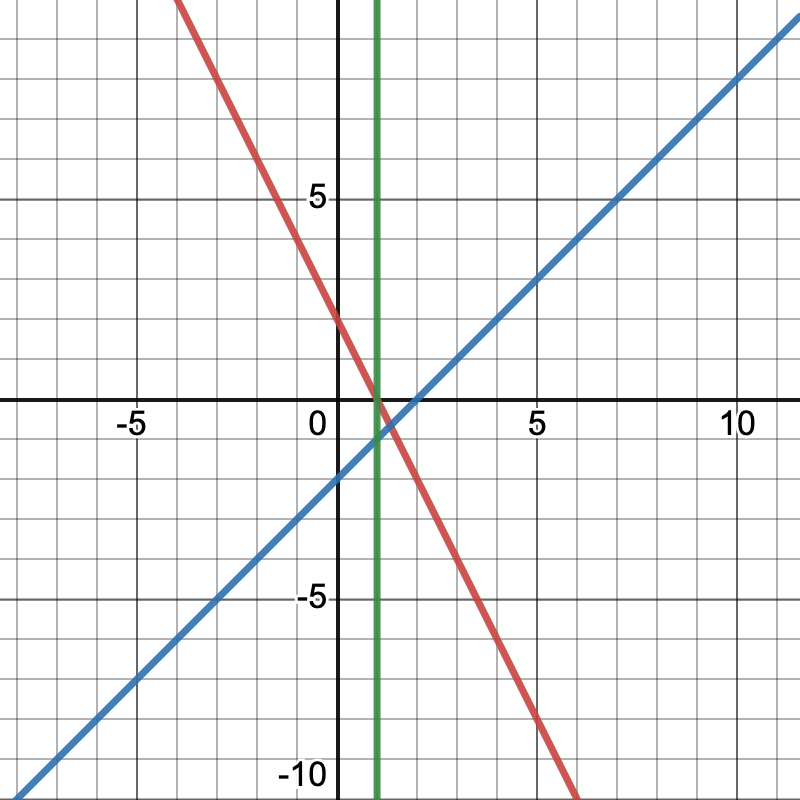
\includegraphics{h1q5s1.png}

    No solution.\\
    \questionpart
    \begin{equation}
        \begin{cases}
            2x+y&=2\\
            x-y&=2\\
            x&=\frac{4}{3}
        \end{cases}
    \end{equation}
        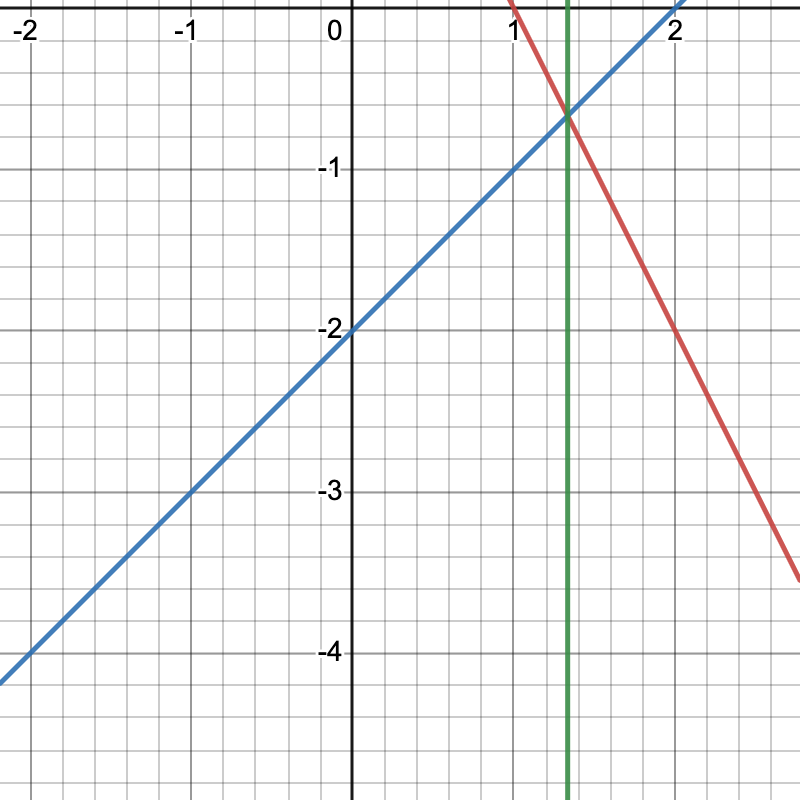
\includegraphics{h1q5s2.png}


    
    \end{arabicparts}
    \question
    \begin{equation}
        \left[\begin{array}{cccc}
        \hlight{a} & 1 & 3 & r \\ 
        a & a & 4 & s \\ 
        a & a & 2a & t
        \end{array}\right]
        \to
        \left[\begin{array}{cccc}
        \hlight{a} & 1 & 3 & r \\ 
        0 & a-1 & 1 & s-r \\ 
        0 & a-1 & 2a-3 & t-r
        \end{array}\right]
    \end{equation}
    when $a\neq0$, the elimination fails to give the pivot.
    \begin{equation}
        \left[\begin{array}{cccc}
            \hlight{a} & 1 & 3 & r \\ 
            0 & a-1 & 1 & s-r \\ 
            0 & a-1 & 2a-3 & t-r
            \end{array}\right]
        \to
        \left[\begin{array}{cccc}
        a & 1 & 3 & r \\ 
        0 & \hlight{a-1} & 1 & s-r \\ 
        0 & 0 & 2a-4 & t-s
        \end{array}\right]
    \end{equation}
    when $a\neq1$, the elimination fails to give the pivot.
    \begin{equation}
        \left[\begin{array}{cccc}
            a & 1 & 3 & r \\ 
            0 & a-1 & 1 & s-r \\ 
            0 & 0 & \hlight{2a-4} & t-s
            \end{array}\right]
    \end{equation}
    when $a\neq2$, the elimination fails to give the pivot.

    Hence,
    \begin{equation}
        a=\begin{cases}
            0\\
            1\\
            2
        \end{cases}
    \end{equation}

    \question
    By
    \begin{equation}
        ab^T=
        \left[\begin{array}{cccc}
        39 & 99 & 420 & 207 \\ 
        45 & 33 & 782 & 199 \\ 
        100 & 80 & 49 & 73 \\ 
        59 & 18 & 75 & 46
        \end{array}\right]
        =
        \left[\begin{array}{cccc}
        a_1 b_1 & a_1 b_2  & a_1 b_3  & a_1 b_4  \\ 
        a_2 b_1  & a_2 b_2  & a_2 b_3  & a_2 b_4  \\ 
        a_3 b_1  & a_3 b_2  & a_3 b_3  & a_3 b_4  \\ 
        a_4 b_1  & a_4 b_2  & a_4 b_3  & a_4 b_4 
        \end{array}\right]
    \end{equation}
    we could get
    \begin{equation}
        a^Tb=a_1 b_1 + a_2 b_2 + a_3 b_3 + a_4 b_4=39+33+49+46=167
    \end{equation}

    \question
    \begin{multline}
        A^3=(ab^T)^3=
        (\begin{bmatrix}
        1 \\ 
        2 \\ 
        3
        \end{bmatrix}
        \cdot
        \left[\begin{array}{ccc}
        1 & 1 & 0
        \end{array}\right]
        )^3=
        \left[\begin{array}{ccc}
        1 & 1 & 0 \\ 
        2 & 2 & 0 \\ 
        3 & 3 & 0
        \end{array}\right]^3\\
        =
        \left[\begin{array}{ccc}
        1 & 1 & 0 \\ 
        2 & 2 & 0 \\ 
        3 & 3 & 0
        \end{array}\right]
        \left[\begin{array}{ccc}
        3 & 3 & 0 \\ 
        6 & 6 & 0 \\ 
        9 & 9 & 0
        \end{array}\right]=
        \left[\begin{array}{ccc}
        9 & 9 & 0 \\ 
        18 & 18 & 0 \\ 
        27 & 27 & 0
        \end{array}\right]
    \end{multline}
    
    
    \question
    Given
    \begin{align}
        (I-xy^T)^{-1}&=(I+xy^T)\\
        (I-xy^T)(I-xy^T)^{-1}&=(I-xy^T)(I+xy^T)\\
        (I-xy^T)(I-xy^T)^{-1}&=I^2-xy^T+xy^T+(xy^T)^2\\
        I&=I+x(y^Tx)y^T\\
        0&=x(y^Tx)y^T\label{eq25}
        % x^Ty &=a_1 b_1 +a_2 b_2 + a_3 b_3 + a_4 b_4\\
        % y^Tx &=a_1 b_1 +a_2 b_2 + a_3 b_3 + a_4 b_4\\
        % x^Ty &=0
    \end{align}
    % , it follows that
    % \begin{equation}
    %     y^Tx=x^Ty=0
    % \end{equation}
    % By eq. (24),
    % it is not hard to find that
    % \begin{align}
    %     (I-xy^T)^{-1}&=(I+xy^T)\\
    %     ((I-xy^T)^{-1})^T&=((I+xy^T))^T
    % \end{align}
    if $y^Tx=0$, then \cref{eq25} is true. 
    \question
    \begin{equation}
        C^n=B^{-1}ABB^{-1}AB\dots B^{-1}ABB^{-1}AB=B^{-1}\underbrace{A\dots A}_{\text{n times}}B=B^{-1}A^nB
    \end{equation}
\end{document}

